%\begin{comment}
\documentclass[a4paper,11pt]{article}
\usepackage{graphicx}
\usepackage[brazilian]{babel}
\usepackage[latin1]{inputenc}
\usepackage[T1]{fontenc}
\usepackage{fullpage}
\begin{document}
%\end{comment}

\section{Arquitetura do Sistema de Localiza��o}

O sistema de localiza��o estima a posi��o do rob� a partir dos dados de seus sensores. No SAURON, os sensores s�o os oito sonares e uma c�mera de v�deo. Cada sensor tem associado a si um modelo de observa��o, que descreve a rela��o da medida lida com o mundo real. Por exemplo, o modelo de observa��o do sonar associa uma s�rie de leituras a uma parede no mapa. De agora em diante, quando falarmos em um sensor, estamos nos referindo ao seu modelo de observa��o.

Cada sensor sabe qual � a observa��o esperada para uma dada postura do rob�. Uma diferen�a entre a observa��o esperada e a observa��o de fato recebida indica um erro na estimativa do sistema. Se esses erros forem pequenos, podem ser consequ�ncia das varia��es naturais dos sensores f�sicos. Contudo, diferen�as grandes devem ser utilizadas para corrigir a postura estimada. O ponto mais importante do algoritmo de localiza��o � exatamente este: a partir da diferen�a entre as observa��es esperadas e reais, atualizar a estimativa da postura.

Essas estimativas, que s�o corrigidas pelos sensores, s�o geradas pelo mo


\begin{figure}
	\centering
		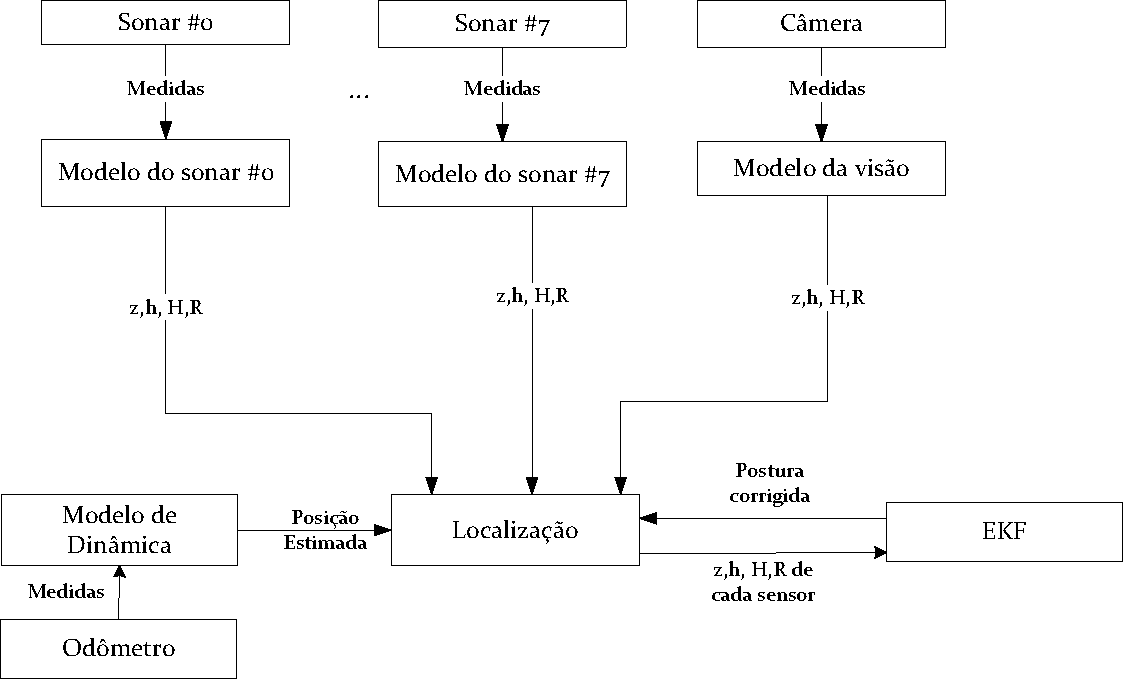
\includegraphics[width=.8\columnwidth]{imagens/arquitetura.pdf}
	\caption{Modelo refinado de incid�ncia dos sonares. $\beta=\theta_{sonar}+\alpha$}
	\label{fig:nossomodelo}
\end{figure}

\end{document}